% Mirror: https://github.com/SIGma-UIUC/presentation-format
% --------------------------------------------------------------------
% This is a simple Beamer document that uses beamerthemesigma.sty
% Reading the comments should help you create a presentation even if
% you've never used Beamer before.
% --------------------------------------------------------------------

% Set our document class to Beamer
\documentclass[aspectratio=169]{beamer}
% \documentclass[aspectratio=169, handout]{beamer}
% Add handout option to ignore pauses

% From Jeff E
\usepackage{algo}
% Some more macros
\usepackage{sigmastyle}
\usepackage{colortbl}
\usepackage{xcolor}
\usepackage{array}

% Set a title
\title{World's Simplest Poker}

% Set a subtitle if you desire

% Whoever worked on the presentation:
\author{Mihir Tandon}

% Date looks ugly, so leave blank
\date{}

% An institute name, if you're so inclined
% \institute{University of Illinois Urbana-Champaign}

% Use the SIGma theme for this Beamer presentation
\usetheme{sigma}
% --------------------------------------------------------------------

% Begin document
\begin{document}

% Beamer calls each slide a "frame", defined within the environment:
% \begin{frame}
%   <frame content here>
% \end{frame}

% This frame is just the title.
\begin{frame}
\titlepage
\end{frame}

% A frame with the table of contents.
% This frame's title is "Outline".
% Start a section: *sections* (subsections, etc.) are what show up in the TOC.
\begin{frame}{Disclaimer}
    \begin{itemize}
        \item This presentation is based on an IML (Illinois Mathematics Lab) project I am working on, ``The Mathematics of Poker-Like Games", under Professor  Hildebrand.
        \item The IML project is inspired by \href{https://cheaptalk.org/wp-content/uploads/2012/11/worlds-simplest-poker.pdf}{``World's Simplest Poker"} (2012) by Professor David McAdams of Duke University.
        \item As we are still researching, some ideas in this presentation remain open/not fully explored.
        \item I might do a (short) presentation later in the semester exploring these ideas.
        \item The point of this talk is not to teach you the best poker strategy or make you a better poker player.
    \end{itemize}
\end{frame}
\begin{frame}{Outline}
  \tableofcontents
  \end{frame}
\section{Introduction}
% Section pages can be printed thus:
\frame{\sectionpage}
% There's a way to automate this, see:
% https://tex.stackexchange.com/questions/178800/creating-sections-each-with-title-pages-in-beamers-slides/178803

\begin{frame}{World's Simplest Poker}
    \begin{itemize}
        \item \textit{Poker} is a game of betting, luck and strategy. \pause
        \item 
         We consider a (very) simplified version of poker, in which there are two players A and B, and $n$ cards labeled 1 to $n.$\pause
        \item Each player is dealt a random card without replacement.\pause
        \item The initial ante to play is $\$1,$ then players can choose to \textit{bet} an additional $\$1$ or \textit{fold}, independently of the other player's choice.\pause
        \item If one player bets, and the other folds, that player wins $\$1.$ \pause
        \item If both players fold, the player with the higher card wins $\$1.$ \pause
        \item If both players bet, the player with the higher card wins $\$2.$ \pause
        \item Note that ``fold'' doesn't mean losing the hand right away!
        
        
        %\textcolor{sigma@mainblue}{colors} \textcolor{sigma@highlightpink}{are} \textcolor{sigma@alertred}{cool}
    \end{itemize}
\end{frame}
\begin{frame}{Example Game}
%  \item  \textcolor{sigma@mainblue}{colors} \textcolor{sigma@highlightpink}{are} \textcolor{sigma@alertred}{cool}
  \frametitle{Example Game}
  % Some fun with LaTeX Math
  \begin{itemize}
  \item Let $n=3.$ (This is often referred to as \textit{A-K-Q Poker}), and that the other player bets if and only if they get card $2$ or $3.$ \pause
  \item Suppose you get a $1.$ Should you bet? \pause  
    \\ \textit{Answer:} No \pause
  \item Suppose you get a $3.$ Should you bet?  \pause
    \\ \textit{Answer:} Yes \pause
  \item Suppose you get a $2.$ Should you bet?  \pause 
    \\ \textit{Answer:} No \pause
  \item $\mathbb E$ from betting: $\mathbb{E}_2 = 1 \cdot \frac{1}{2} - 2\cdot \frac{1}{2} = -\frac{1}{2}.$
  \item $\mathbb E$ from not betting: $\mathbb{E}_2 = 1 \cdot \frac{1}{2} - 1\cdot \frac{1}{2} = 0.$
  \pause
  \item Note that we consider a player's strategy \textit{independently} of the other player's bet. For all we know, the could be bluffing!
\end{itemize}
\end{frame}
\begin{frame}{More Examples}
\begin{itemize}
 \item Define a player's \textit{betting set} $S_A, S_B \subseteq \{1,2,3,\ldots,n\}$ ($S_A$ for player $A,$ $S_B$ for player $B$)  such that a player bets on card $c$ if and only if $c \in S_A, S_B.$ \pause
    \item Suppose player A has a betting set $S_A = \{\}.$  What is player B's best response? \pause
     \\ \textit{Answer:} $S_B = \{1,2,3\}.$ Player $B$ will always win!
    \end{itemize}
    \end{frame}
\begin{frame}{More Examples}
\begin{itemize}
 \item Suppose player A has a betting set $S_A = \{1,2,3\}.$ What is player B's best response? \pause
    \\ \textit{Answer:}
    \begin{itemize}
    \item You should always bet on 3, never on 1. \pause
    \item If you bet on 2, your expected payout is $\mathbb{E}_2 = 2\cdot \frac{1}{2}-2\cdot\frac{1}{2} = 0.$\pause
    \item If you fold on 2, your expected payout is $\mathbb{E}_2 =-\frac{1}{2}-\frac{1}{2} = -1,$ since $A$ always bets. \pause
    \item Thus, $S_A = \{2,3\}.$
\end{itemize}
\end{itemize}
\end{frame}
\begin{frame}{Game Theory Fundamentals}
\begin{itemize}
   \item A \textit{zero-sum} game has a expected payout sum over all players of 0. Poker is, of course, a zero-sum game. \pause
   \item We say a player has a \textit{dominant strategy} if it is the best strategy for the player, regardless of what the other player chooses to do.\pause
    \item We call a strategy  \textit{deterministic} if it always produces the same outcome for a given input, without any randomness or uncertainty (We have only considered deterministic strategies so far).
    \pause
    \item A \textit{Nash Equilibrium} occurs when neither player can gain a higher payout by changing their current strategy.
\end{itemize}
\end{frame}
\begin{frame}{Payout Matrix for $n=3$}
\begin{itemize}
\item We can compute all of the results for $n=3,$ (either by hand or python code simulating all the games in $\mathcal{O}(2^{n}\cdot 2^{n} \cdot n^2) = \mathcal{O}(4^{n}n^{2})$ time)\pause
 \item What would dominant strategies or Nash Equilibria look like in this table? \pause
\end{itemize}
\begin{table}[H]
    \centering
    \begin{tabular}{|c|c|c|c|c|c|c|c|c|}
        \hline
        $S_B \backslash S_A$ & \{\} & \{1\} & \{2\} & \{3\} & \{1,2\} & \{1,3\} & \{2,3\} & \{1,2,3\} \\ 
        \hline
        \{\}      & 0  & 4  & 2  & 0  & 6  & 4  & 2  & 6 \\ \hline 
        \{1\}      & -4 & 0  & 1  & -1 & 5  & 3  & 4  & 8  \\ \hline 
        \{2\}      & -2 & -1 & 0  & 1  & 1  & 2  & 3  & 4  \\ \hline 
        \{3\}      & 0  & 1  & -1 & 0  & 0  & 1 & -1 & 0  \\ \hline 
        \{1,2\}    & -6 & -5 & -1 & 0  & 0  & 1  & 5  & 6  \\ \hline 
        \{1,3\}    & -4 & -3 & -2 & -1 & -1 & 0  & 1  & 2  \\ \hline 
        \{2,3\}    & -2 & -4 & -3 & 1  & -5 & -1 & 0  & -2 \\ \hline 
        \{1,2,3\}  & -6 & -8 & -4 & 0  & -6 & -2 & 2  & 0  \\ \hline 
        \hline
    \end{tabular} 
   \caption{Player A Payoff matrix for A and B strategies for $n=3$}
\end{table}
\end{frame}
\begin{frame}{Payout Matrix for $n=3$}
  \begin{itemize}
      \item That's right, there are none! We will continue to explore this idea later...
  \end{itemize}
\end{frame}
% Use \pause to make stuff readable
% Large walls of text scare the audience, we don't want that
% Introducing stuff sequentially allows for questions
% \begin{frame}
%   % Alternate syntax for frame titles
%   \frametitle{There Is No Largest Prime Number}
%   % Frames can have subtitles:
%   \framesubtitle{The proof uses \textit{reductio ad absurdum}.}
%   % Some frame content:
%   \begin{thrm}
%     There is no largest prime number.
%   \end{thrm}
%   \begin{pf}
%     \begin{enumerate}
%         \item Suppose $p$ were the largest prime number \pause
%         \item Let $q$ be the product of the first $p$ primes \pause
%         \item Then $q+1$ is not divisible by any of them \pause
%         \item But $q + 1$ is greater than $1$, thus divisible by some prime number not in the first $p$ numbers. \pause
%         \item Thus, there exists a prime larger than $p$.
%     \end{enumerate}
%   \end{pf}
% \end{frame}

% However, this doesn't work in math mode. It is quite annoying to figure out
% So just copy this as reference
% This works for \onslide<> and \item<>
% Really good read on this: 
%   https://www.texdev.net/2014/01/17/the-beamer-slide-overlay-concept/
%\begin{frame}{Sequential Math Frames}
 %   Here is a sentence \pause
    
  %  I shall now carry out some calculations \pause
   % \begin{align*}
    %    \onslide<+->{\zeta(s) &= \sum_{n = 1}^\infty \frac{1}{n^s} \\}
%    %     \onslide<+->{&= \prod_{p \in \text{primes}} \frac{1}{1 - p^{-s}} \\}
%         \onslide<.->{&= \frac{1}{1 - 2^-s} \cdot \frac{1}{1 - 3^-s} \cdots \\}
%         \onslide<+->{&= \frac{1}{\Gamma(s)} \int_0^\infty \frac{x^{s - 1}}{e^x - 1} ~\textrm{d}x\\}
%     \end{align*}
% \end{frame}

\section{The Cutoff Strategy}
\frame{\sectionpage}
\begin{frame}{The Cutoff Strategy}
\begin{itemize}
    \item A common deterministic strategy players use is called the \textit{cutoff} strategy, where a player bets if and only the card $c_i$ they receive is greater than or equal to a certain cutoff value $1 \leq A_c,B_c \leq n+1.$ \pause
    \item What would be the betting set of a player using a cutoff strategy of $A_c = 2$? (Assume $n=3$). \pause
    \\ \textit{Answer:} $S_A = \{2,3\}.$
\end{itemize}
\end{frame}
\begin{frame}{Analysis of The Cutoff Strategy}
\begin{itemize}
\item Using this subset of all possible deterministic strategies, we can find the expected payout of each player given their cutoff values $A_c, B_c$ and $n.$ \pause
\item WLOG, assume that $A_c > B_c.$ We find a formula for player A's expected payout $\mathbb{E}_A$ and use the zero-sum game fact as $\mathbb{E}_A = - \mathbb{E}_B.$ \pause
\item What about when $A_c = B_c$? What is $\mathbb{E}_A$ in this case? \pause
\\ \textit{Answer:} By symmetry, $ \mathbb{E}_A = \mathbb{E}_B = 0.$
\end{itemize}
\end{frame}
\begin{frame}{Analysis of The Cutoff Strategy}
\begin{itemize}
\item We end up with 6 cases to consider: 
\begin{enumerate}
        \item FFL
        \item FFW
        \item BFW
        \item FBL
        \item BBW
        \item BBL
    \end{enumerate}
\item The first letter is player A's action (fold or bet), the second letter is player B's action (fold or bet), and the last letter is the outcome for the case for player A (win or lose). \pause
\item What happened to the BFL and FBW cases? \pause
\textit{Answer:} If player A bets and player B folds, player A always wins. 

\end{itemize}
\end{frame}
\begin{frame}{}
    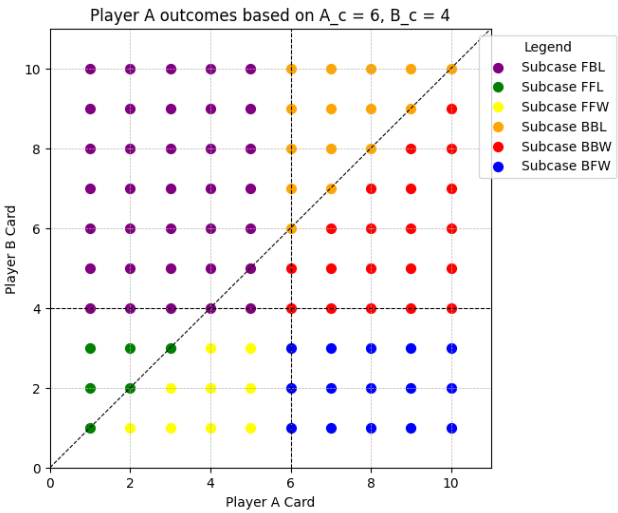
\includegraphics[scale=0.6]{DiscreteCutoffs.png}
\end{frame}
\begin{frame}{Analysis of the Cutoff Strategy}
\begin{itemize}
\item The total expected payout is then: $$\mathbb{E}_A = \sum_{i=1}^{6}\mathbb{E}_{\text{case \#i}} \cdot P_{\text{case \#i}},$$
where $\mathbb{E}_\text{case \#i}$ and $P_{\text{case \#i}}$ are the expected profit and probability given that $x$ and $y$ satisfy the relations for case $\#i.$
\item In this presentation, I will only go through one case, as the derivation is similar for the other five.
\end{itemize}
\end{frame}
\begin{frame}{The FFL Case}
\begin{itemize}
\item  This case arises in the scenario that neither player bets and Player A loses the showdown. \pause
\item  First, we compute the probability that this case occurs. \pause
    \item Let $c_A$ and $c_B$ be the card players A and B recieve, respectively. There are $n \cdot (n-1)$ ways to choose $c_A$ and $c_B.$ \pause
    \item There are $(B_c-1)$ ways to pick $c_B < B_c$. \pause
    \item Since player A loses this hand, we need $c_A < c_B < B_c$ as well, and there are $(B_c-2)$ cards left satisfying $c_A < B_c.$ \pause
    \item By symmetry, exactly $1/2$ of these cases satisfy $c_A < c_B.$ \pause
    \item Thus, we get $$P_{1} = \frac{(B_c-1)(B_c-2)}{2n(n-1)}.$$ 
\end{itemize}
\end{frame}
\begin{frame}{The FFL Case}
    \begin{itemize}
        \item Note that $\mathbb{E}_{\text{case \#1}} = -1,$ as player A loses the showdown and neither player bets. Thus, we have $$\mathbb{E}_{\text{case \#1}} \cdot P_{\text{case \#1}} = -1 \cdot \frac{(B_c-1)(B_c-2)}{2n(n-1)} = -\frac{(B_c-1)(B_c-2)}{2n(n-1)}.$$
    \end{itemize}
\end{frame}
\begin{frame}{The other cases}
\begin{itemize}
    \item Doing the same for the other 5 cases, we find the following results: \begin{tabular}{|c|c|c|}
\hline
Case & Player A Profit & Probability  \\ 
\hline 
\hline
BBW & +2 & $\frac{(n+1-A_c)(n+A_c-2B_c)}{2n(n-1)}$ \\
\hline
BBL & -2 & $\frac{(n+1-A_c)(n-A_c)}{2n(n-1)}$  \\  
\hline
FFW & +1 & $\frac{(B_c-1)(2A_c-B_c-2)}{2n(n-1)}$ \\
\hline
FFL & -1 & $\frac{(B_c-1)(B_c-2)}{2n(n-1)}$ \\
\hline
BFW & +1 & $\frac{(n-A_c+1)(B_c-1)}{n(n-1)}$ \\
\hline
FBL & -1 & $\frac{(A_c-B_c)(n-B_c)+(B_c-1)(n-B_c+1)}{n(n-1)}$ \\
\hline
\end{tabular}
\end{itemize}
\end{frame}
\begin{frame}{Putting it all together}
\begin{itemize} 
    \item Going through the messy algebra, we eventually get that $$\mathbb{E}_A = \sum_{i=1}^{6}\mathbb{E}_{\text{case \#i}} \cdot P_{\text{case \#i}} \Longrightarrow$$ $$ \mathbb{E}_A =\frac{3A_cB_c-B_c^2-2A_c^2+2A_c-2B_c+nA_c-nB_c}{n(n-1)},\{A_c > B_c\}.$$ 
    \item Since we have a zero-sum game, we have $$\mathbb{E}_B = -\mathbb{E}_A = \frac{-3A_cB_c+B_c^2+2A_c^2-2A_c+2B_c-nA_c+nB_c}{n(n-1)},\{A_c>B_c\}.$$
    \end{itemize}
\end{frame}
\begin{frame}{Putting it all Together}
\begin{itemize}
    \item Since the game is symmetric between the two players, we can swap all of the indices $A$ and $B$ to derive the case when $B_c > A_c.$ $$\mathbb{E}_A = \frac{-3A_cB_c+A_c^2+2B_c^2-2B_c+2A_c-nB_c+nA_c}{n(n-1)},\{B_c > A_c\}.$$
    \item Thus, we have found a (pretty ugly) formula for player A's expected payout given both cutoffs $A_c,$ $B_c,$ and $n.$ 
    \end{itemize}
\end{frame}
\begin{frame}{MatPlotlib Python Plot}
    \begin{figure}
        \centering
        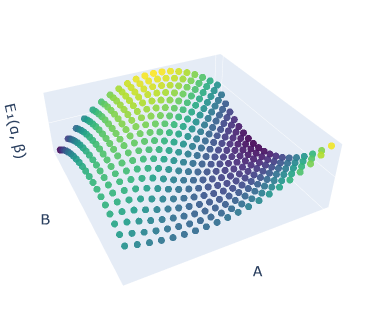
\includegraphics[scale=0.8]{3dplot.png}
        \caption{Expected Payoff of Player 1 in terms of cutoffs $A$ and $B$}
        \label{fig:enter-label}
    \end{figure}
\end{frame}
\begin{frame}{Level Curves}
    \begin{itemize}
        \item To better visualize this 3D space, we can plot \textit{level curves}, where we hold $B_c$ constant and plot $\mathbb{E}$ vs. $A_c$:
\begin{figure}
        \centering
        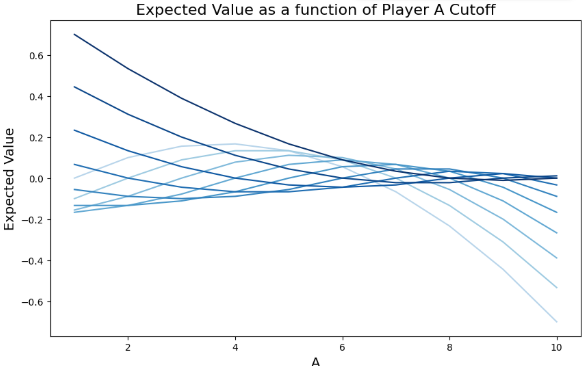
\includegraphics[scale=0.5]{levelcurves.png}
    \end{figure} \item Darker curves indicate larger values of $B_c.$
        \end{itemize}
\end{frame}
\begin{frame}{Finding Player 1's Maximum Payout}
    \begin{itemize}
        \item We now maximize $\mathbb{E}_A$ over $A_c$ for a fixed $B_c$ and $n.$ \pause
        \item  Suppose that player $A$ adopts a strategy with $A_c > B_c.$  \pause
        \item Then player $1$'s expected payout is given by $$\mathbb{E}_A = \frac{3A_cB_c-B_c^2-2A_c^2+2A_c-2B_c+nA_c-nB_c}{n(n-1)}.$$ \pause
        \item We re-write this as a quadratic in $A_c:$ $$\mathbb{E}_A = \frac{-2A_c^2+(2+n+3B_c)A_c-(B_c^2+nB_c+2B_c)}{n(n-1)}.$$ \pause
        \item Then, we take the derivative with respect to $A_c$ ($B_c$ is fixed) $$\frac{\partial}{\partial A_c}\mathbb{E}_A = \frac{-4A_c+(2+n+3B_c)}{n(n-1)}$$ 
        \end{itemize}
    \end{frame}
 \begin{frame}{Finding Player 1's Maximum Payout $(A_c > B_c)$}
    \begin{itemize}
        \item This function has a maximum at $$\frac{\partial}{\partial A_c}(\mathbb{E}_A) = 0 \Longrightarrow\frac{-4A_c+(2+n+3B_c)}{n(n-1)} = 0 \Longrightarrow A_c^{*}=\frac{2+n+3B_c}{4}.$$ \pause
        \item We can verify that $A_c^{*}$ satisfies $B_c <A_c^{*} \leq n+1,$ for all $1 \leq B_n \leq n+1,$ so this choice of $A_c=A_c^{*}$ is valid. \pause
        \item Thus, an optimal choice of $A_c$ for strategies satisfying $A_c > B_c$ is $$A^{*}_c = \left \lfloor \frac{2+n+3B_c}{4} \right \rceil,$$ where $\lfloor x \rceil$  is the closest integer function. 
    \end{itemize}
    \end{frame}
\begin{frame}{Finding Player 1's Maximum Payout $(A_c < B_c)$}
\pause
    \begin{itemize}
        \item We have $$\mathbb{E}_A =\frac{A_c^2+(n+2-3B_c)A_c-(nB_c+2B_c-2B_c^2)}{n(n-1)}.$$ \pause
        \item Since this parabola opens up, we consider the endpoints. $A_C = \{1,B_1-1\}.$ \pause
        \item $A_c=1$: We have $$\mathbb{E}_A =\frac{1^2+(n+2-3B_c)\cdot 1-(nB_c+2B_c-2B_c^2)}{n(n-1)} \Longrightarrow $$$$\mathbb{E}_A =\frac{3+n-5B_c-nB_c+2B_c^2}{n(n-1)}.$$ 
    \end{itemize}
\end{frame}
\begin{frame}{Finding Player 1's Maximum Payout $(A_c > B_c)$}
\begin{itemize}
      \item $A_c=B_c-1$: We have $$\mathbb{E}_A =\frac{(B_c-1)^2+(n+2-3B_c)(B_c-1)-(nB_c+2B_c-2B_c^2)}{n(n-1)} \Longrightarrow$$ \pause
       $$ \mathbb{E}_A=\frac{B_c-n-1}{n(n-1)}.$$ \pause
      \item But since $B_c \leq n+1,$ we have $ \mathbb{E}_A\leq0$ in this case, so player $A$ would never choose this strategy. 
\end{itemize}
\end{frame}
\begin{frame}{Finding Player 1's Maximum Payout}
\begin{itemize}
    \item Thus, given $B_c,$ the optimal value of $A_c$ is either $1$ or $\left \lfloor \frac{2+n+3B_c}{4} \right \rceil,$ depending on which gives a larger value for $\mathbb{E}_A.$ \pause
    \item In general, player A should use $A_c = 1$ while $B_c$ is high, then switch to $\left \lfloor \frac{2+n+3B_c}{4} \right \rceil$ when player B's cutoff gets low enough. \pause
    \item Finding the exact value for when to switch is quite annoying due to the closest integer function. \pause
    \item Instead, we find a useful approximation that lets us drop the closest integer.
    \end{itemize}
\end{frame}
\begin{frame}{The Continuous Analog}
\begin{itemize}
    \item As $n$ grows large, we can ignore the discrete differences in cards, the without replacement condition, (and drop the closest integer function). \pause
    \item Recall that $n$ is the number of potential \textit{hands}, so for a 52 card deck, this could be as large as ${52 \choose 2} = 1326.$ \pause
    \item Then, we can reframe our problem as choosing cutoffs $\alpha_c$ and $\beta_c$ such that $\alpha_c,\beta_c \in \mathbb{R}$ and $\alpha_c,\beta_c  \in [0,1],$ and frame the cards chosen as random real numbers in $[0,1].$ \pause
    \item We can derive the continuous versions of our formulas by approximating $B_c \approx n\beta_c,$ $A_c \approx n\alpha_c,$ and taking the limit as $n \to \infty.$ 
\end{itemize}
\end{frame}
\begin{frame}{The Continuous Analog - Expected Profit}
\begin{itemize}
    \item Substituting \( A_c = n\alpha_c \) and \( B_c = n\beta_c \) into the formula for $\mathbb{E}_A$ (assuming $\beta_c > \alpha_c$), we obtain
\[
\mathbb{E}_A = \frac{2\beta_c^2 n^2 - (n+2+3n\alpha_c)n\beta_c + (n^2\alpha_c^2 + (n+2)n\alpha_c)}{n(n-1)}
\] \pause
\item Taking the limit as $n \to \infty,$ only the quadratic terms survive. 
 \[
\lim_{n \to \infty} \mathbb{E}_A = \lim_{n \to \infty} \frac{n^2(2\beta_c^2 - \beta_c - 3\alpha_c\beta_c + \alpha_c^2 + \alpha_c)}{n(n-1)} = 2\beta_c^{2}-\beta_c-3\alpha_c\beta_c+\alpha_c^{2}+\alpha_c.
\] \pause
\item We can similarly derive $\mathbb{E}_A$ in the case $\alpha_c > \beta_c$: $$\mathbb{E}_A = -2\alpha_c ^2 -\beta_c ^2 + 3\alpha_c\beta_c + \alpha_c - \beta_c$$
\end{itemize}
\end{frame}
\begin{frame}{The Continuous Analog - Maximization}
\pause
\begin{itemize}
    \item We can compute the $\alpha_c^{*}$ (best cutoff values for player $A$ as $n \to \infty),$ rescaling to $[0,1],$ using our formulas from before. \pause
    $$A^{*}_c = 1 \Longrightarrow \alpha^{*}_c=0, \{\alpha_c < \beta_c\}$$ \pause
    $$A^{*}_c = \left \lfloor \frac{2+n+3B_c}{4} \right \rceil \Longrightarrow \alpha^{*}_c = \frac{3\beta+1}{4}, \{\alpha_c > \beta_c\}$$ \pause
    \item Plugging these back to $\mathbb{E}_A$: \pause$$\mathbb{E}_A(0) =2\beta_c^{2}-\beta_c,\{\alpha_c < \beta_c\}.$$ \pause
 $$\mathbb{E}_A\left(\frac{3\beta+1}{4}\right)  = \frac{(\beta_c - 1)^2}{8},\{\alpha_c > \beta_c\}.$$
\end{itemize}
\end{frame}
\begin{frame}{The Continuous Analog - Maximization}
\begin{itemize}
    \item Now, we find for which $\beta_c$ we should choose $\alpha^{*}=0$ or $\alpha^{*}=\frac{3\beta+1}{4}.$ \pause $$\mathbb{E}_A(0) > \mathbb{E}_A\left(\frac{3\beta+1}{4}\right) \Longleftrightarrow 2\beta_c^{2}-\beta_c > \frac{(\beta_c-1)^{2}}{8}$$\pause $$\Longleftrightarrow 15\beta_c^{2}-6\beta_c-1>0 \Longleftrightarrow \beta_c >\frac{3+2\sqrt{6}}{15} \approx 0.5266.$$ \pause
    \item Thus, player $A$ should play with a cutoff strategy $\alpha = 0$ iff $\beta_c > \frac{3+2\sqrt{6}}{15},$ otherwise player A should use a cutoff of $\frac{3\beta+1}{4}.$ \pause
    \item If player $B$ chooses their best strategy with $\beta_c^{*} = \frac{3+2\sqrt{6}}{15},$ then player $A$ can achieve a maximum expected payout of $$\mathbb{E}_A = \frac{(\beta_c^{*}-1)^2}{8} = \frac{7-2\sqrt{6}}{75} \approx 0.028.$$ 
\end{itemize}
\end{frame}
\begin{frame}{The Continuous Analog - Graph}
\begin{figure}
    \centering
    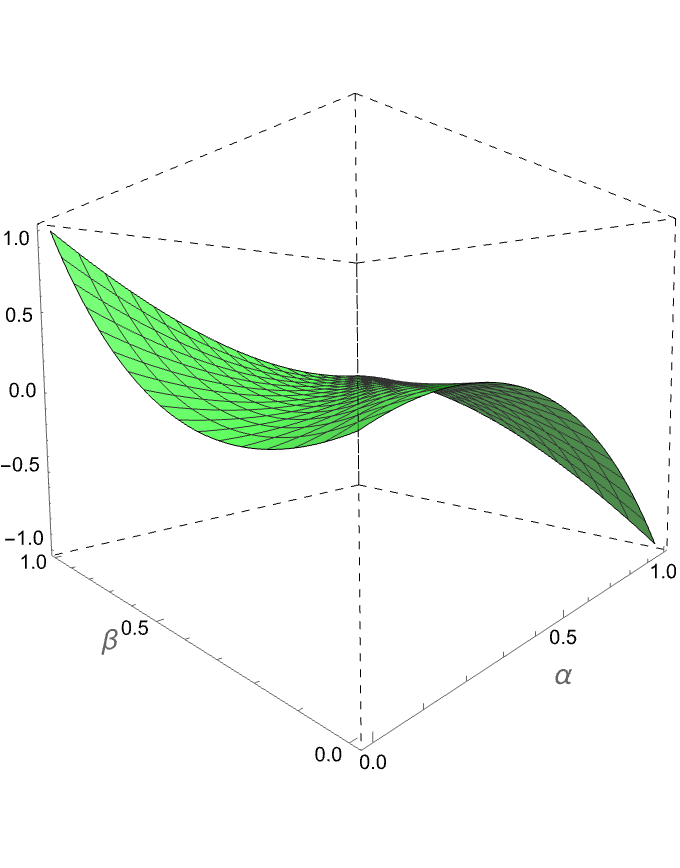
\includegraphics[scale=0.6]{3DGraph.png}
\end{figure}
\end{frame}
% Similar for subsections:
% \subsection{A subsection, Wow}
% % And their pages:
% \frame{\subsectionpage}

% \begin{frame}{Image}
%   % This is how you'd include an image, centered.
%   \begin{center}
%     
\includegraphics[width=0.25\textwidth]{sigma.png}
%   \end{center}
% \end{frame}

% \begin{frame}{Side by Side}
%     
\includegraphics[width=0.25\textwidth]{sigma.png}\hspace{0.4\textwidth}
%     
\includegraphics[width=0.25\textwidth]{sigma.png}
% \end{frame}

% \begin{frame}{Demonstration of algo and nalgo env}
%     \begin{algo}
%     \underline{\textsc{GetRandomNumber}():}\+
%     \\      return $4$   \Comment{chosen by fair dice roll.}
%     \\      \hspace{42.75pt}\Comment{guaranteed to be random.}
%     \end{algo}
    
%     % nalgo has line numbers
%     % only lines with \label{} are numbered
%     \begin{nalgo}[1.3]
%         \underline{\textsc{GetRandomNumber}():}\+
%     \\\label{}  return $4$   \Comment{chosen by fair dice roll.}
%     \\\label{}  \hspace{42.75pt}\Comment{guaranteed to be random.}
%     \end{nalgo}
    
%     Random number generation from~\cite{site:xkcd}. 
%     \quest{
%     \textbackslash cref for line numbers does not work. 
%     If you want to refer to specific line numbers, do it manually
%     }
    
% \end{frame}

% \begin{frame}{}
% \begin{minipage}[c]{0.6\textwidth}
% \begin{nalgo}
% \textul{\textbf{\textsc{AlgorithmP}}$(S[a_0, \dots, a_n])$}:
% \\\label{}  $C[1..n] \gets 0, O[1..n] \gets 1$
% \\\label{}  \textbf{while} \textsc{True}:\+
% \\\label{}      \textsc{print}$(S)$
% \\\label{}      {\color{lightgray}$j \gets n, s \gets 0$}
% \\\label{}      {\color{lightgray}\textbf{A:}~~$q \gets C[j] + O[j]$\+}
% \\\label{}          {\color{lightgray}\textbf{if} $q < 0$: goto \textbf{D}}
% \\\label{}          {\color{lightgray}\textbf{if} $q = j$: goto \textbf{B}}
% \\\label{}          {\color{lightgray}\textsc{swap}$(S, j-C[j]+s, j-q+s)$}
% \\\label{}          {\color{lightgray}$C[j] \gets q$} 
% \\\label{}          {\color{lightgray}continue\-}
% \\\label{}      {\color{lightgray}\textbf{B:}~~\textbf{if} $j=1$:\+\+}
% \\\label{}              {\color{lightgray}break\-}
% \\\label{}          {\color{lightgray}$s \gets s+1$\-}
% \\\label{}    {\color{lightgray}\textbf{D:}~~$O[j] \gets -O[j], j \gets j-1$\+}
% \\\label{}      {\color{lightgray}goto \textbf{A}}
% \end{nalgo}
% \end{minipage}
% \begin{minipage}[c]{0.35\textwidth}
% \begin{itemize}
%     \item Here is an example of annotating an algorithms \pause
%     \item We have grayed out text to highlight what we want to discuss 
% \end{itemize}
% \end{minipage}
% \end{frame}

% Of course, not everything is in pseudocode
% You MUST have this [containsverbatim] option
% https://www.overleaf.com/learn/latex/Code_Highlighting_with_minted
% \begin{frame}[containsverbatim]{Source Code}
%     \begin{minted}
%     [
%     framesep=2mm,
%     baselinestretch=1.2,
%     bgcolor=black,
%     fontsize=\footnotesize,
%     ]
%     {python}
%     def algorithm_g(n):
%         a = [0 for _ in range(n + 1)]
%         while True:
%             curr = a[1 : n + 1][::-1]
%             yield "".join([str(i) for i in curr])
    
%             a[0] = 1 - a[0]
%             j = 1
%             while a[j - 1] != 1:
%                 j += 1
%             if j == n + 1:
%                 return
%             a[j] = 1 - a[j]
%     \end{minted}
% \end{frame}


% \begin{frame}{Theorems and Lemmas}
%     \begin{lem}
%         The map $\C \times \pqty{\C \setminus \set{0}} \to \C$, $(z, w) \mapsto z / w$ is $C^{\infty}$.
%     \end{lem}
%     \begin{pf}
%         To see this, we identify $\C$ with $\R^{2}$ where $a + bi = (a, b)$.
%         Thus our map is now
%         \begin{align*}
%             \pqty{\R^{2}} \times \pqty{\R^{2} \setminus \set{(0, 0)}} &\to \R^{2} \\
%                             ((a, b), (c, d)) &\mapsto \pqty{\frac{ac + bd}{c^{2} + d^{2}}, \frac{bc - ad}{c^{2} + d^{2}}}
%         \end{align*}
%         which is well defined since at least one of $c$ or $d$ is nonzero.
%         It is simple to verify that this map is equivalent to the original one.
%         Since this new map is $C^{\infty}$ in each component, we have that it is $C^{\infty}$ overall.
%     \end{pf}
% \end{frame}
\section{General Strategies}
% Section pages can be printed thus:
\frame{\sectionpage}
\begin{frame}{Dominance of Deterministic Strategies}
\begin{itemize}
    \item Up until now, we have focused on analyzing the cutoff strategy and the expected payouts gained from it. \pause
    \item But is the cutoff strategy a dominant strategy? 
    \pause
    \item That is, no matter what player B does, can player A achieve their maximum possible expected profit by using a cutoff strategy?
\end{itemize}
\end{frame}
\begin{frame}{Dominance of Deterministic Strategies}
\begin{itemize}
      \item Consider $S_B = \{3\}.$ (Recall that $S_B$ is the \textit{betting set} of player $B$). \pause
    \item What is player $A$'s best response? \pause
    \begin{table}[H]
    \centering
    \begin{tabular}{|c|c|c|c|c|c|c|c|c|}
        \hline
        $S_B \backslash S_A$ & \{\} & \{1\} & \{2\} & \{3\} & \{1,2\} & \{1,3\} & \{2,3\} & \{1,2,3\} \\ 
        \hline
        \{\}      & 0  & 4  & 2  & 0  & 6  & 4  & 2  & 6 \\ \hline 
        \{1\}      & -4 & 0  & 1  & -1 & 5  & 3  & 4  & 8  \\ \hline 
        \{2\}      & -2 & -1 & 0  & 1  & 1  & 2  & 3  & 4  \\ \hline 
        \{3\}      & 0  & 1  & -1 & 0  & 0  & 1 & -1 & 0  \\ \hline 
        \{1,2\}    & -6 & -5 & -1 & 0  & 0  & 1  & 5  & 6  \\ \hline 
        \{1,3\}    & -4 & -3 & -2 & -1 & -1 & 0  & 1  & 2  \\ \hline 
        \{2,3\}    & -2 & -4 & -3 & 1  & -5 & -1 & 0  & -2 \\ \hline 
        \{1,2,3\}  & -6 & -8 & -4 & 0  & -6 & -2 & 2  & 0  \\ \hline 
        \hline
    \end{tabular} 
   \caption{Payoff matrix for A and B strategies}
\end{table}
\end{itemize}
\end{frame}
\begin{frame}{Dominance of Deterministic Strategies}
\begin{itemize}
    \item Answer: $S_A = \{1\}$ or $\{1,3\}$... hey wait, neither of those are cutoff strategies! \pause
    \item It follows that only playing cutoff strategies is not optimal, and there are situations where other strategies are better. \pause
    \item However, it can be shown that a cutoff strategy is optimal for (nearly all) possible bluffing sets of the other player.
    \pause
    \item Thus, the cutoff strategy is still ``generally" good.
\end{itemize}
\end{frame}
\begin{frame}{Repeated Iterations of Optimal Strategies}
\begin{itemize}
    \item Consider this scenario: \pause
    \begin{itemize}
    \item Player $A$ picks a strategy $S_A$ \pause
    \item Player $B$ picks their optimal response $S_B$ \pause
    \item Player $A$ then changes their strategy to pick their best possible response given player $B$s current strategy. \pause
    \item Then player $B$ changes their strategy, and the cycle repeats. \pause
\end{itemize}
    \item This leads to a sequence of iterated strategies, which we will call $s_1,s_2,s_3,\ldots,s_T.$ \pause
    \item Note that this sequence must eventually be periodic, as there are only finitely many possible values of $s_i,$ and $s_{i+1}$ only depends on the value of $s_i.$  \pause
    \item Let's call the period of such a ``strategy cycle" $T.$
    \end{itemize}
    \end{frame}
    \begin{frame}{Repeated Iterations of Optimal Strategies}
    \begin{itemize}
    \item Question: What other term refers to a strategy cycle of length 1 (i.e. $T=1$)? \pause
    \textit{Answer:} A Nash Equilibrium!
    \end{itemize}
    \end{frame}
    \begin{frame}{Repeated Iterations of Optimal Strategies}
    \begin{itemize}
    \item For example, suppose $n=3$ and initially player B bets 
    on $S_B = \{2,3\}.$ \pause 
  \begin{tabular}{|c|c|c|c|c|c|c|c|c|}
        \hline
        $S_B \backslash S_A$ & \{\} & \{1\} & \{2\} & \{3\} & \{1,2\} & \{1,3\} & \{2,3\} & \{1,2,3\} \\ 
        \hline
        \{\}      & 0  & 4  & 2  & 0  & 6  & 4  & 2  & 6 \\ \hline 
        \{1\}      & -4 & 0  & 1  & -1 & 5  & 3  & 3  & 8  \\ \hline 
        \{2\}      & -2 & -1 & 0  & 1  & 1  & 2  & 3  & 4  \\ \hline 
        \{3\}      & 0  & 1  & -1 & 0  & 1  & -1 & -1 & 0  \\ \hline 
        \{1,2\}    & -6 & -5 & -1 & 0  & 0  & 1  & 5  & 6  \\ \hline 
        \{1,3\}    & -4 & -3 & -2 & -1 & -1 & 0  & 1  & 2  \\ \hline 
        \{2,3\}    & -2 & -4 & -3 & \only<3->{\cellcolor{cyan}}1  & -5 & -1 & 0  & -2 \\ \hline 
        \{1,2,3\}  & -6 & -8 & -4 & 0  & -6 & -2 & 2  & 0  \\ \hline 
        \hline
    \end{tabular} 
    \item What is player $A's$ best response? \pause 
    Answer: $S_A = \{3\}.$ 
    \end{itemize}
    \end{frame}
    \begin{frame}{Repeated Iterations of Optimal Strategies}
    \begin{tabular}{|c|c|c|c|c|c|c|c|c|}
    \hline
    $S_B \backslash S_A$ & \{\} & \{1\} & \{2\} & \{3\} & \{1,2\} & \{1,3\} & \{2,3\} & \{1,2,3\} \\ 
    \hline
    \{\}      & 0  & 4  & 2  & 0  & 6  & 4  & 2  & 6 \\ \hline 
    \{1\}      & -4 & 0  & 1  & -1 & 5  & 3  & 3  & 8  \\ \hline 
    \{2\}      & -2 & -1 & 0  & 1  & 1  & 2  & 3  & 4  \\ \hline 
    \{3\}      & 0  & 1  & -1 & 0  & 1  & -1 & -1 & 0  \\ \hline 
    \{1,2\}    & -6 & -5 & -1 & 0  & 0  & 1  & 5  & 6  \\ \hline 
    \{1,3\}    & -4 & -3 & -2 & \only<2->{\cellcolor{yellow}}-1 & -1 & 0  & 1  & 2  \\ \hline 
     \{2,3\}  & -2 & -4 & -3 & \cellcolor{cyan}1  & -5 & -1 & 0  & -2 \\ \hline 
    \{1,2,3\}  & -6 & -8 & -4 & 0  & -6 & -2 & 2  & 0  \\ \hline 
    \hline
    \hline
\end{tabular}
\begin{itemize}
    \item Now, what would player B do to maximize their payout?\pause
    \item Player B would bet on $\{1\}$ or  $\{1,3\}.$ (It turns out it doesn't matter which one is picked, so we assume $S_B = \{1,3\}$ in this case.)
    \end{itemize}
\end{frame}
\begin{frame}{Repeated Iterations of Optimal Strategies}
\begin{itemize}
    \item We can continue this process until we arrive back at where we started. \pause
    \begin{tabular}{|c|c|c|c|c|c|c|c|c|}
    \hline
    $S_B \backslash S_A$ & \{\} & \{1\} & \{2\} & \{3\} & \{1,2\} & \{1,3\} & \{2,3\} & \{1,2,3\} \\ 
    \hline
    \{\}      & 0  & 4  & 2  & 0  & 6  & 4  & 2  & 6 \\ \hline 
    \{1\}      & -4 & 0  & 1  & -1 & 5  & 3  & 3  & 8  \\ \hline 
    \{2\}      & -2 & -1 & 0  & 1  & 1  & 2  & 3  & 4  \\ \hline 
    \{3\}      & 0  & 1  & -1 & 0  & 1  & -1 & -1 & 0  \\ \hline 
    \{1,2\}    & -6 & -5 & -1 & 0  & 0  & 1  & 5  & 6  \\ \hline 
    \{1,3\}    & -4 & -3 & -2 & \cellcolor{yellow}-1 & -1 & 0  & 1  & \only<3->{\cellcolor{green}}2  \\ \hline 
     \{2,3\}  & -2 & -4 & -3 & \cellcolor{cyan}1  & -5 & -1 & 0  & \only<4->{\cellcolor{red}}-2 \\ \hline 
    \{1,2,3\}  & -6 & -8 & -4 & 0  & -6 & -2 & 2  & 0  \\ \hline 
    \hline
    \hline
\end{tabular}
\only<5->{\item The cycle now repeats. Thus, the period is $T=4.$}
   \end{itemize}
\end{frame}
\begin{frame}{Repeated Iterations of Optimal Strategies}
\begin{itemize}
\item We know that there are cycles of length $4$ for all $n \leq 10,$ as well as cycles of length $10$ for $n \geq 4.$ \pause
\item However, we have yet to prove that these are the only ones yet.
   \end{itemize}
\end{frame}
\begin{frame}{Bluffing}
\begin{itemize}
\item A common \textit{non-deterministic} strategy is   \textit{bluffing.} \pause
\item A player with card $c,$ betting cutoff $A,$ and bluffing probability $p$ will bet with probability $p$ if $c < A,$ and always bet with $c \geq A.$ \pause
\item We haven't looked to much into this, but it has been shown that, in the continuous case, if both players have the same betting cutoff and bluffing probability, there is a nash equilibrium at $$(p_A,A_c)=(p_B,B_C)=\left(\frac{1}{3},\frac{1}{2}\right),$$  due to David McAdams (2012).
\end{itemize}
\end{frame}
\begin{frame}{Future Work}
\begin{itemize}
\item There are several questions we have yet to answer, here are some of the most pressing mysteries. \pause
\item Given that player $B$ chooses a betting set $S_B,$ what is player $A$'s best possible response, in terms of $S_B$? \pause
\item Does there exist a nash equilbrium in the discrete case considering deterministic strategies? \pause
\item Are there any nash equilbria or dominant strategies when bluffing is introduced? \pause
\item We hope to find some answers to these questions as we continue our research.
\end{itemize}
\end{frame}
    \begin{frame}{Python Code}
    \begin{itemize}
        \item \href{https://colab.research.google.com/github/aryan-cs/poker-like-games/blob/discrete-poker/discrete_poker_games.ipynb\#scrollTo=rYfmVTdfblIf}{Link to Colab Notebook}
    \end{itemize}
\end{frame}
% Asking questions is fun but we should answer some first
\begin{frame}{}
      \begin{center}
    {\color{sigma@mainblue} \LARGE Questions?}
  \end{center}
\end{frame}

\begin{frame}{Brainteaser}
\begin{itemize}
    \item Let $S$ be the set of all distinct triangles (i.e, no two triangles in $S$ are congruent) that have perimeter $2025$ and integer degree angle measures. A random triangle is chosen from $S$. What is the probability that the selected triangle is obtuse? 
    \end{itemize}
\end{frame}

% Quotes are fun, find some to use!
\font\eightss=cmssq8
\font\eightssi=cmssqi8
\newcommand\quoteAuthorDate[3]{\begingroup
  \baselineskip 10pt
  \parfillskip 0pt
  \interlinepenalty 10000 % not needed in example
  \leftskip 0pt plus 40pc minus \parindent
  \let\rm=\eightss
  \let\sl=\eightssi
  \everypar{\sl}#1\par
  \nobreak\smallskip
  \noindent\rm--- #2\unskip\enspace(#3)\par
  \endgroup}
% If someone can figure out how to horizontally center this and make the text bigger that'd be cool

% Remove this slide if you came up with all the material yourself
\begin{frame}[allowframebreaks]{Bibliography}
    \tiny
    \bibliography{refs}
    \bibliographystyle{alpha}
\begin{itemize}
    \item McAdams, David. "World's Simplest Poker" \textit{Duke University,} 2013, \href{https://cheaptalk.org/wp-content/uploads/2012/11/worlds-simplest-poker.pdf}{https://cheaptalk.org/wp-content/uploads/2012/11/worlds-simplest-poker.pdf}
\end{itemize}
\end{frame}

\end{document}